\documentclass{beamer}

\usepackage{tikz}
\usepackage{xcolor}
\usepackage{csquotes}
\usepackage{pgfplots}
\pgfplotsset{compat=1.18}
\usetikzlibrary{shapes, positioning}
\definecolor{keywordcolor}{rgb}{0.7, 0.1, 0.1}   % red
\definecolor{commentcolor}{rgb}{0.4, 0.4, 0.4}   % grey
\definecolor{symbolcolor}{rgb}{0.0, 0.1, 0.6}    % blue
\definecolor{sortcolor}{rgb}{0.1, 0.5, 0.1}      % green
\usepackage{listings, lstautogobble}
\def\lstlanguagefiles{lstlean.tex}
\lstset{
    language=lean,
    autogobble=true,
    escapeinside={(.}{.)},
}

\newcommand{\mathcolorbox}[2]{\colorbox{#1}{$\displaystyle #2$}}

\addtobeamertemplate{navigation symbols}{}{%
    \usebeamerfont{footline}%
    \usebeamercolor[fg]{footline}%
    \hspace{1em}%
    \insertframenumber/\inserttotalframenumber
}

\author{Johannes Tantow}
\title{LEAN-Aided Certification of Datalog Reasoning Results}
\date{05.06.2024}
\usetheme{Dresden}


\begin{document}
    \maketitle

    \section{Introduction}
    \begin{frame}{Introduction} 
      

        \begin{tikzpicture}[node distance=2.5cm and 20cm, auto]
    
            \tikzstyle{block} = [rectangle, minimum width=2cm, minimum height=1cm]
            \tikzstyle{database} = [cylinder,
            shape border rotate=90,
            aspect=0.25,
            draw]

            \node[database] (db) at (0,4) {Database};
            
            \node[draw, align=center] (program) at (0,0) {
            \begin{minipage}{4cm}
              \begin{align*}
                T(?x,?y) \leftarrow &E(?x,?y). \\ T(?x,?z) \leftarrow &T(?x,?y),\\ &E(?y, ?z) .
              \end{align*}
            \end{minipage}
          };

          \node[block, draw] (engine) at (4,2) {Datalog engine};

          \node[block, align=left] (result) at (8,2) {Result: \\ $\{T(1,3), \dots \}$};

          \draw[->] (engine) -- (result);
          \draw[->] (program) |- (engine);
          \draw[->] (db) |- (engine);            
        \end{tikzpicture}
    \end{frame}

    \begin{frame}{Tracing}
      \begin{tikzpicture}
        \node (A) at (0,0) {T(0,2)};
        \node (B) at (-1, -2) {T(0,1)};
        \node (C) at (1,-2) {E(1,2)};
        \node (D) at (-1, -4) {E(0,1)};

        \draw [->] (A) -- (B);
        \draw [->] (A) -- (C);
        \draw[->] (B) -- (D);

        \node (trace) at (7, 0) {Trace: T(0,2)};

        \node[rectangle, draw] (engine) at (7, -2) {Datalog engine};

        \node[draw, align=center] (program) at (7,-4) {
            \begin{minipage}{4cm}
              \begin{align*}
                T(?x,?y) \leftarrow &E(?x,?y). \\ T(?x,?z) \leftarrow &T(?x,?y),\\ &E(?y, ?z) .
              \end{align*}
            \end{minipage}
          };
        
        \draw[->] (program) -- (engine);
        \draw[->] (trace) -- (engine);
        \draw [->] (engine) -- (2.5, -2);


      \end{tikzpicture}
    \end{frame}

    \begin{frame}{Lean}
        \resizebox{.9\textwidth}{!}{
        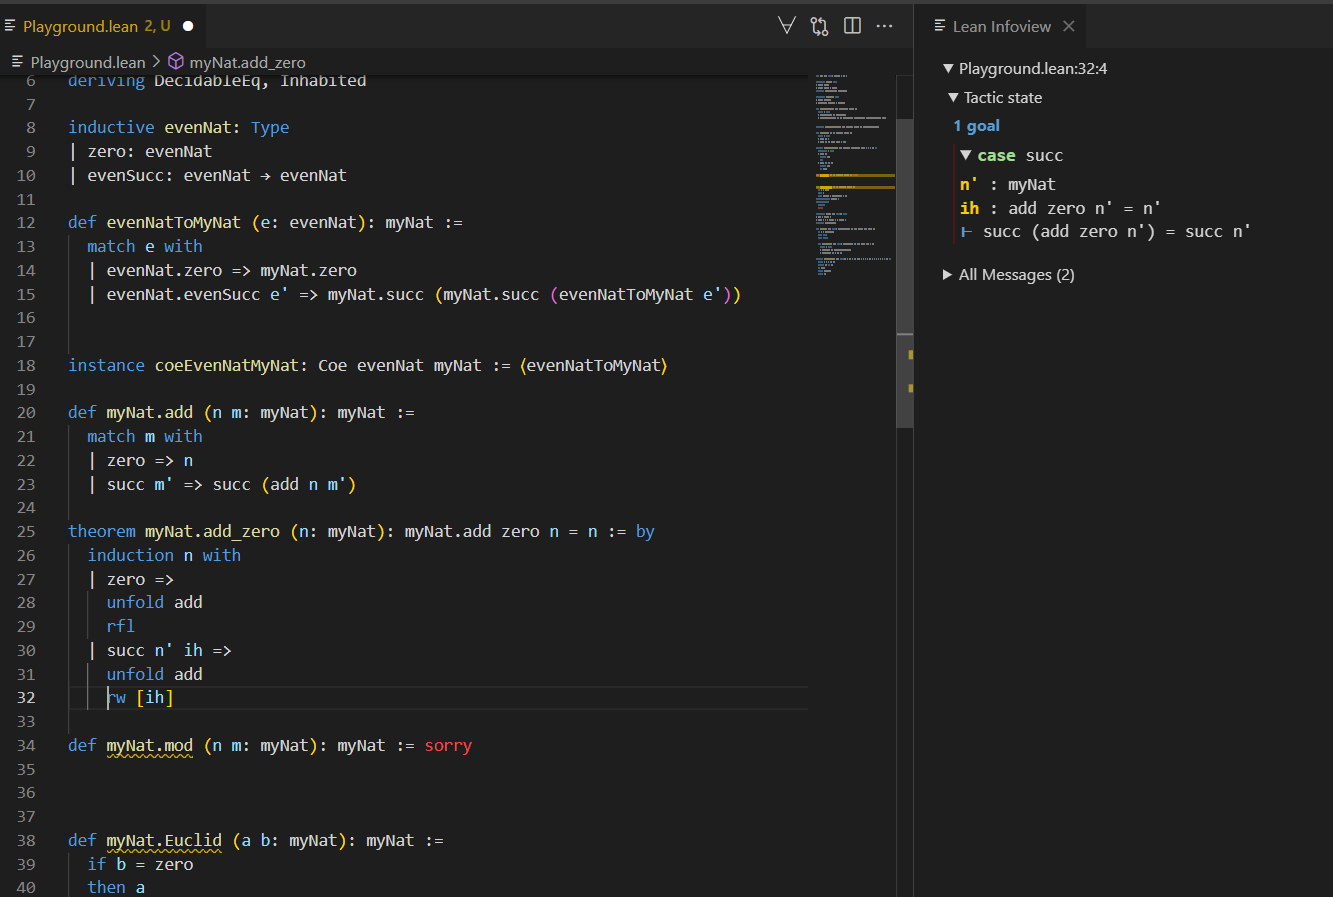
\includegraphics{Lean_example2.png}
        }
    \end{frame}

    \begin{frame}{Outline}
      \begin{enumerate}
        \item Formalize datalog
        \item Soundness: Verify datalog proofs
        \item Completeness: Can more be derived?
        \item Evaluation
      \end{enumerate}
      
    \end{frame}

    \section{Formalizing Datalog}

    \begin{frame}[fragile]{Syntax}
      \begin{center}
      \resizebox{!}{0.8\textheight}{
      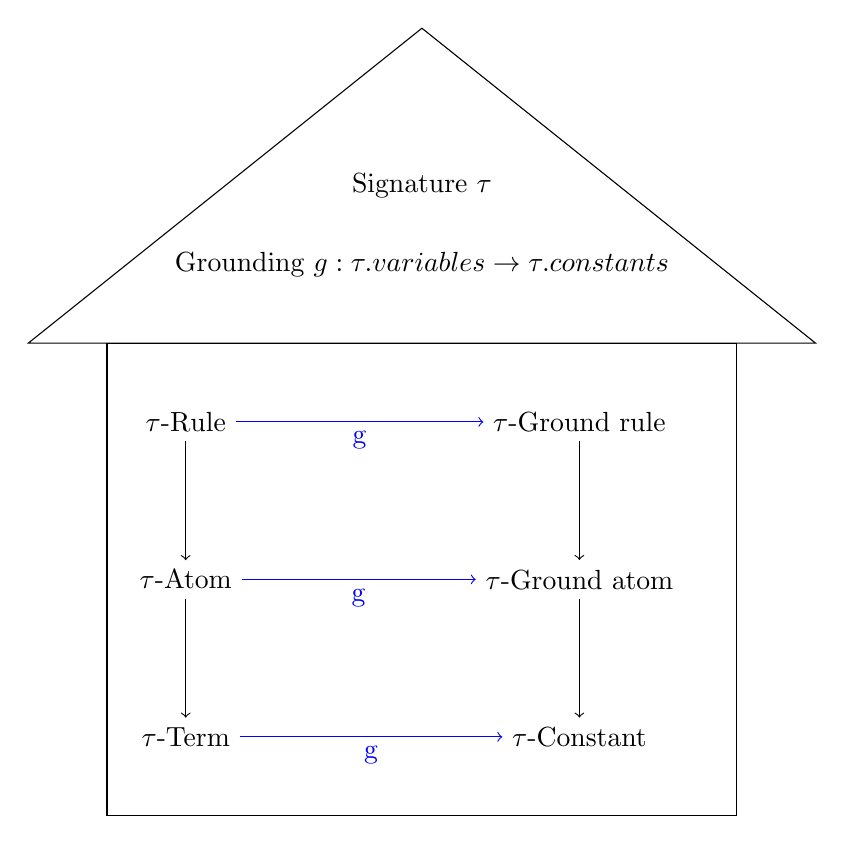
\begin{tikzpicture}

        % Draw the house base (rectangle)
        \draw[] (0,0) rectangle (8,6);

        \node (Term) at (1,1) {$\tau$-Term};
        \node (Atom) at (1,3) {$\tau$-Atom};
        \node (Rule) at (1,5) {$\tau$-Rule};

        \node (GroundTerm) at (6,1) {$\tau$-Constant};
        \node (GroundAtom) at (6,3) {$\tau$-Ground atom};
        \node (GroundRule) at (6,5) {$\tau$-Ground rule};

        % Draw the roof (triangle)
        \draw[] (4,10) -- (-1,6) -- (9,6) -- cycle;

        \node (Signature) at (4,8) {Signature $\tau$};
        \node (Grouding) at (4,7) {Grounding $g: \tau.variables \to \tau.constants$};

        \draw[<-] (Term) -- (Atom);
        \draw[<-] (Atom) -- (Rule);
        \draw[<-] (GroundTerm) -- (GroundAtom);
        \draw[<-] (GroundAtom) -- (GroundRule);

        \draw[->,blue] (Term) -- (GroundTerm) node[pos=0.5, below] {g};
        \draw[->,blue] (Atom) -- (GroundAtom) node[pos=0.5, below] {g};
        \draw[->,blue] (Rule) -- (GroundRule) node[pos=0.5, below] {g};

      \end{tikzpicture}
      }
      \end{center}
    \end{frame}

    \begin{frame}[fragile]{Model-theoretic semantics}
      \begin{definition}[12.2.1, Alice Book]
        Let $P$ be a datalog program. \textelp{} The semantics of $P$ on input $I$, denoted
        $P (I)$, is the minimum model of $P$ containing $I$, if it exists.
      \end{definition}

      \pause
      \[M = \bigcap_{X \text{ is model of } P}  X \]
      \pause

      \begin{lstlisting}
            def iInter (s : ι → Set α) : Set α
      \end{lstlisting}
      \pause

      \[ M = \{a \in \text{ groundAtom } \tau \mid \forall i, \text{isModel i P} \rightarrow a \in i\} \]
    \end{frame}

    \begin{frame}[fragile]{Proof-theoretic semantics}
      \begin{onlyenv}<1>
        
      \begin{columns}
      \begin{column}{.3\textwidth}
        
      
      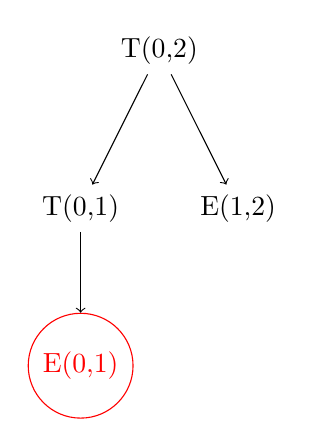
\begin{tikzpicture}
        \node (A) at (0,0) {T(0,2)};
        \node (B) at (-1, -2) {T(0,1)};
        \node (C) at (1,-2) {E(1,2)};
        \node[circle, draw, red] (D) at (-1, -4) {E(0,1)};

        \draw [->] (A) -- (B);
        \draw [->] (A) -- (C);
        \draw[->] (B) -- (D);
      \end{tikzpicture}
      \end{column}
      \begin{column}{.6\textwidth}
        Database contains $E(0,1)$.
      \end{column}
    \end{columns}

  \end{onlyenv}

  \begin{onlyenv}<2>
        
    \begin{columns}
    \begin{column}{.3\textwidth}
      
    
    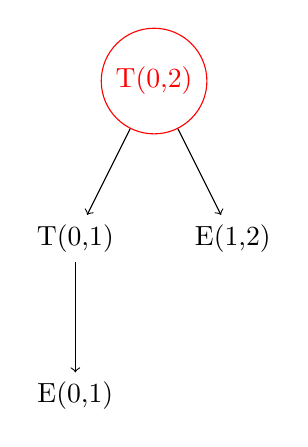
\begin{tikzpicture}
      \node[circle, draw, red] (A) at (0,0) {T(0,2)};
      \node (B) at (-1, -2) {T(0,1)};
      \node (C) at (1,-2) {E(1,2)};
      \node (D) at (-1, -4) {E(0,1)};

      \draw [->] (A) -- (B);
      \draw [->] (A) -- (C);
      \draw[->] (B) -- (D);
    \end{tikzpicture}
    \end{column}
    \begin{column}{.6\textwidth}
      $\exists r, g$:

      \begin{enumerate}
        \item $r\in P$
        \item $T(0,2) \leftarrow T(0,1), E(1,2) = apply(r,g)$
        \item All subtrees are valid
      \end{enumerate}
    \end{column}
  \end{columns}

\end{onlyenv}

    \end{frame}

    \section{Soundness}

    \begin{frame}{Unification}

      \begin{center}
        \resizebox{!}{0.8\textheight}{
        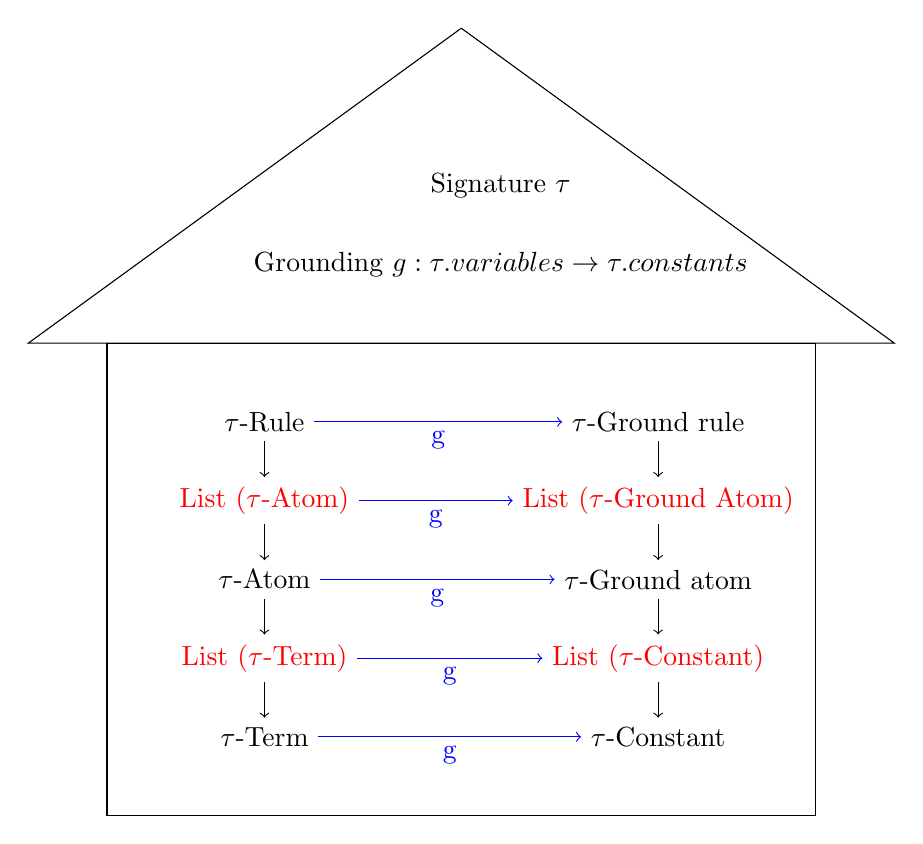
\begin{tikzpicture}
            \draw[] (-1,0) rectangle (8,6);
  
          \node (Term) at (1,1) {$\tau$-Term};
          \node (ListTerm) at (1,2) {\textcolor{red}{List ($\tau$-Term)}};
          \node (Atom) at (1,3) {$\tau$-Atom};
          \node (ListAtom) at (1,4) {\textcolor{red}{List ($\tau$-Atom)}};
          \node (Rule) at (1,5) {$\tau$-Rule};
  
          \node (GroundTerm) at (6,1) {$\tau$-Constant};
          \node (ListGroundTerm) at (6,2) {\textcolor{red}{List ($\tau$-Constant)}};

          \node (GroundAtom) at (6,3) {$\tau$-Ground atom};
          \node (ListGroundAtom) at (6,4) {\textcolor{red}{List ($\tau$-Ground Atom)}};

          \node (GroundRule) at (6,5) {$\tau$-Ground rule};
  
          % Draw the roof (triangle)
          \draw[] (3.5,10) -- (-2,6) -- (9,6) -- cycle;
  
          \node (Signature) at (4,8) {Signature $\tau$};
          \node (Grouding) at (4,7) {Grounding $g: \tau.variables \to \tau.constants$};
  
          \draw[<-] (ListTerm) -- (Atom);
          \draw[<-] (Term) -- (ListTerm);
          \draw[<-] (Atom) -- (ListAtom);
          \draw[<-] (ListAtom) -- (Rule);
          \draw[<-] (ListGroundTerm) -- (GroundAtom);
          \draw[<-] (GroundTerm) -- (ListGroundTerm);
          \draw[<-] (GroundAtom) -- (ListGroundAtom);
          \draw[<-] (ListGroundAtom) -- (GroundRule);
  
          \draw[->,blue] (Term) -- (GroundTerm) node[pos=0.5, below] {g};
          \draw[->,blue] (ListTerm) -- (ListGroundTerm) node[pos=0.5, below] {g};

          \draw[->,blue] (Atom) -- (GroundAtom) node[pos=0.5, below] {g};
          \draw[->,blue] (ListAtom) -- (ListGroundAtom) node[pos=0.5, below] {g};

          \draw[->,blue] (Rule) -- (GroundRule) node[pos=0.5, below] {g};
  
        \end{tikzpicture}
        }
        \end{center}
      
    \end{frame}

    \begin{frame}[fragile]{Substitutions}
      \only<1>{
      \begin{tabular}{c|cc}
        Terms & $?x$ & $?y$ \\ 
        Ground terms & $a$ & $b$ \\
        \hline
        Groundings & $?x \mapsto a, ?y \mapsto a$ & Error \\
      \end{tabular}
      }

      \begin{onlyenv}<2>
      \begin{tabular}{c|cc}
        Terms & $?x$ & $?y$ \\ 
        Ground terms & $a$ & $b$ \\
        \hline
        Groundings & $?x \mapsto a, ?y \mapsto a$ & Error \\
        Substitutions & $?x \mapsto a$ & $?x \mapsto a, ?y \mapsto b$
      \end{tabular}

      \begin{lstlisting}
        def substitution (τ: signature):= τ.vars → Option (τ.constants)
      \end{lstlisting}
      \end{onlyenv}
    \end{frame}

    \begin{frame}[fragile]{Proof graphs}
      \begin{align*}
        T(?x,?y) &\leftarrow E(?x,?y). \\
        T(?x, ?z) &\leftarrow T(?x,?y), T(?x,?y), E(?y, ?z).
      \end{align*}
      \only<1>{\vspace{3cm}}
        
      \only<2>{
        \begin{center}
      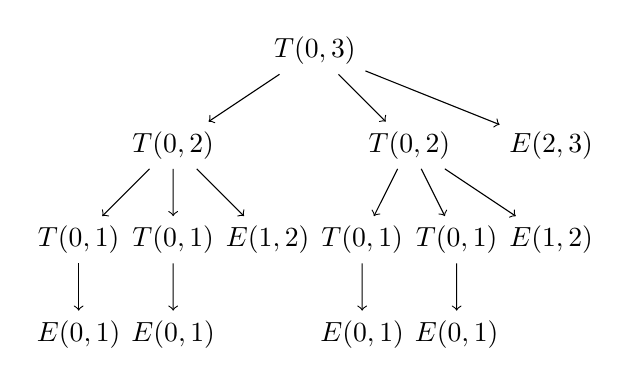
\begin{tikzpicture}[scale=.6]
        \node (A) at (5,4) {$T(0,3)$};
  
        \node (B) at (2,2) {$T(0,2)$};
        \node (C) at (7,2) {$T(0,2)$};
        \node (D) at (10,2) {$E(2,3)$};
  
        \node (E) at (0,0) {$T(0,1)$};
        \node (F) at (2,0) {$T(0,1)$};
        \node (G) at (4,0) {$E(1,2)$};
        \node (H) at (6,0) {$T(0,1)$};
        \node (I) at (8,0) {$T(0,1)$};
        \node (J) at (10,0) {$E(1,2)$};
  
        \node (K) at (0,-2) {$E(0,1)$};
        \node (L) at (2,-2) {$E(0,1)$};
        \node (M) at (6,-2) {$E(0,1)$};
        \node (N) at (8,-2) {$E(0,1)$};
  
        \draw[->] (A) -- (B);
        \draw[->] (A) -- (C);
        \draw[->] (A) -- (D);
        \draw[->] (B) -- (E);
        \draw[->] (B) -- (F);
        \draw[->] (B) -- (G);
        \draw[->] (C) -- (H);
        \draw[->] (C) -- (I);
        \draw[->] (C) -- (J);
        \draw[->] (E) -- (K);
        \draw[->] (F) -- (L);
        \draw[->] (H) -- (M);
        \draw[->] (I) -- (N);
      \end{tikzpicture}
    \end{center}
    }

    \only<3>{
      \begin{center}
        \begin{tikzpicture}[scale=0.9]
          \node[circle] (A) at (0,4) {$T(0,3)$};
          \node[circle] (B) at (-1,2) {$T(0,2)$};
          \node[circle] (C) at (2,2) {$E(2,3)$};
          \node[circle] (D) at (-1,0) {$T(0,1)$};
          \node[circle] (E) at (2,0) {$E(1,2)$};
          \node[circle] (F) at (-1,-2) {$E(0,1)$};
    
          \draw [->] (A) -- (C);
          \draw[->] (A) to[out=235, in=150] (B);
          \draw[->] (A) to[out=280, in=45] (B);
          \draw [->] (B) -- (E);
          \draw[->] (B) to[out=235, in=150] (D);
          \draw[->] (B) to[out=280, in=45] (D);
          \draw[->] (D) -- (F);
        \end{tikzpicture}
      \end{center}
    }

    \end{frame}
    
    \begin{frame}[fragile]{Graphs}
      \begin{onlyenv}<1>
        
      \begin{center}
        
      \begin{tikzpicture}
        \node[circle] (A) at (0,2) {$T(0,3)$};
        \node[circle] (B) at (-2,1) {$T(0,2)$};
        \node[circle] (C) at (1,1) {$E(2,3)$};
        \node[circle] (D) at (-3,0) {$T(0,1)$};
        \node[circle] (E) at (-1,0) {$E(1,2)$};

        \draw (A) -- (B);
        \draw (A) -- (C);
        \draw (B) -- (E);
        \draw (B) -- (D);

      \end{tikzpicture}
      \begin{lstlisting}
        structure SimpleGraph (V : Type u) where
          Adj : V → V → Prop
          symm : Symmetric Adj
      \end{lstlisting}
    \end{center}
  \end{onlyenv}

  \begin{onlyenv}<2>
        
    \begin{center}
      
    \begin{tikzpicture}
      \node[circle] (A) at (0,2) {$T(0,3)$};
      \node[circle] (B) at (-2,1) {$T(0,2)$};
      \node[circle] (C) at (1,1) {$E(2,3)$};
      \node[circle] (D) at (-3,0) {$T(0,1)$};
      \node[circle] (E) at (-1,0) {$E(1,2)$};

      \draw[->] (A) -- (B);
      \draw[<-] (A) -- (C);
      \draw[<-] (B) -- (E);
      \draw[<-] (B) -- (D);

    \end{tikzpicture}
    \begin{lstlisting}
      structure Graph (V : Type u) where
        vertices : List V
        successors: V → List V
    \end{lstlisting}
  \end{center}
\end{onlyenv}

\begin{onlyenv}<3>
        
  \begin{center}
    
  \begin{tikzpicture}
    \node[circle] (A) at (0,2) {$T(0,3)$};
    \node[circle] (B) at (-2,1) {$T(0,2)$};
    \node[circle] (C) at (1,1) {$E(2,3)$};
    \node[circle] (D) at (-3,0) {$T(0,1)$};
    \node[circle] (E) at (-1,0) {$E(1,2)$};

    \draw[->] (A) -- (B);
    \draw[<-] (A) -- (C);
    \draw[<-] (B) -- (E);
    \draw[<-] (B) -- (D);

  \end{tikzpicture}
  \begin{lstlisting}
    def Graph (V: Type) := Std.HashMap V (List V)
  \end{lstlisting}
\end{center}
\end{onlyenv}

    \end{frame}

    \begin{frame}[fragile]{Acyclity criteria}
      Dfs G = true $\Leftrightarrow$ G is acyclic \\
      DfsStep G a = true $\Leftrightarrow$ \dots ?

      \vspace{.5cm}
      \only<1>{
        \begin{tikzpicture}
          \node (A) at (9,0) {A};
          \node (B) at (6,0) {B};
          \node (C) at (3,0) {C};
          \node (D) at (0,0) {D};
      
          \draw[->] (B) -- (A);
          \draw[->] (C) -- (B);
          \draw[->] (A) to [out=165,in=15] (C);
          \draw[->] (D) -- (C);
      
          \node (E) at (0,-3) {E};
          \node (F) at (3, -3) {F};

          \draw[->] (E) -- (F);
        \end{tikzpicture}
      }
      \only<2>{
      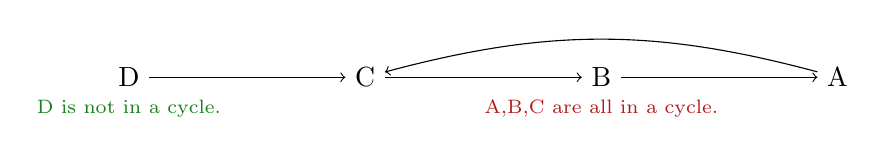
\begin{tikzpicture}
        \node (A) at (9,0) {A};
        \node (B) at (6,0) {B};
        \node (C) at (3,0) {C};
        \node (D) at (0,0) {D};
    
        \draw[->] (B) -- (A);
        \draw[->] (C) -- (B);
        \draw[->] (A) to [out=165,in=15] (C);
        \draw[->] (D) -- (C);
    
        \node at (0,-0.4) {\scriptsize\textcolor{sortcolor}{D is not in a cycle.}};
    
        % \node at (3,-0.4) {\scriptsize\textcolor{keywordcolor}{In Cycle}};
        % \node at (3,-0.7) {\scriptsize\textcolor{keywordcolor}{Reach. from Cycle}};
    
        \node at (6,-0.4) {\scriptsize\textcolor{keywordcolor}{A,B,C are all in a cycle.}};    
        % \node at (9,-0.4) {\scriptsize\textcolor{keywordcolor}{In Cycle}};
        % \node at (9,-0.7) {\scriptsize\textcolor{keywordcolor}{Reach. from Cycle}};
      \end{tikzpicture}
      }
      \only<3>{
      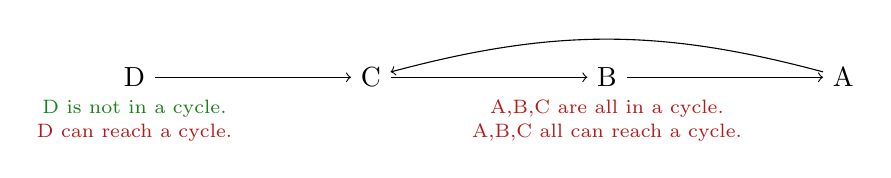
\begin{tikzpicture}
        \node (A) at (9,0) {A};
        \node (B) at (6,0) {B};
        \node (C) at (3,0) {C};
        \node (D) at (0,0) {D};
    
        \draw[->] (B) -- (A);
        \draw[->] (C) -- (B);
        \draw[->] (A) to [out=165,in=15] (C);
        \draw[->] (D) -- (C);
    
        \node at (0,-0.4) {\scriptsize\textcolor{sortcolor}{D is not in a cycle.}};
        \node at (0,-0.7) {\scriptsize\textcolor{keywordcolor}{D can reach  a cycle.}};
    
        % \node at (3,-0.4) {\scriptsize\textcolor{keywordcolor}{In Cycle}};
        % \node at (3,-0.7) {\scriptsize\textcolor{keywordcolor}{Reach. from Cycle}};
    
        \node at (6,-0.4) {\scriptsize\textcolor{keywordcolor}{A,B,C are all in a cycle.}};
        \node at (6,-0.7) {\scriptsize\textcolor{keywordcolor}{A,B,C all can reach  a cycle.}};
    
        % \node at (9,-0.4) {\scriptsize\textcolor{keywordcolor}{In Cycle}};
        % \node at (9,-0.7) {\scriptsize\textcolor{keywordcolor}{Reach. from Cycle}};
      \end{tikzpicture}
      }
    \end{frame}


    \section{Completeness}
    \begin{frame}{Completeness}
      $V$: atoms occurring in the proof graph \\
      $M$: solution

      \vspace{1cm}
      Proof graph valid: $V \subseteq M$
      \pause

      $V$ is a model: $M \subseteq V$ \\
      \vspace{.5cm}
      Hence: $V = M$
    \end{frame}

    \begin{frame}[fragile]{Partial ground rules}
      \[ I = \{ R(a,a,a), R(a,b,c), S(a,b) \}\]
      
        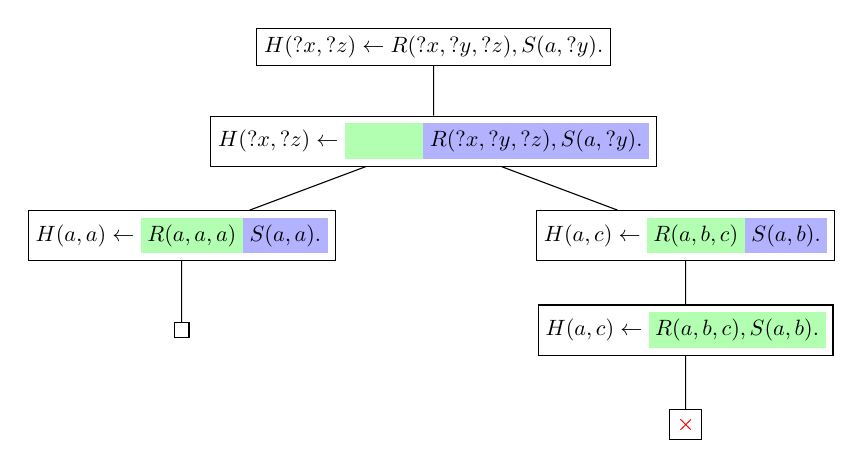
\begin{tikzpicture}[
          scale = 0.8, transform shape,
          every node/.style = {rectangle, draw},
          level distance=1.5cm,
          sibling distance=8cm
        ]
          \node {$H(?x,?z) \leftarrow R(?x,?y,?z), S(a, ?y).$ }
            child {node {$H(?x,?z) \leftarrow \mathcolorbox{green!30}{\phantom{R(a,b)} } \mathcolorbox{blue!30}{R(?x,?y,?z), S(a, ?y).}$}
              child {node {$H(a,a) \leftarrow \mathcolorbox{green!30}{R(a,a,a)} \mathcolorbox{blue!30}{S(a, a).}$} child {node {\textcolor{green}{\checkmark}}}}
              child {node {$H(a,c) \leftarrow \mathcolorbox{green!30}{R(a,b,c)} \mathcolorbox{blue!30}{S(a, b).}$}
                child {node {$H(a,c) \leftarrow \mathcolorbox{green!30}{R(a,b,c), S(a, b).}$} child {node {\textcolor{red}{\texttimes}}} }
              }
            };
  
      \end{tikzpicture}
    \end{frame}

    \section{Evaluation}

    \begin{frame}[fragile]{Soundness \& Completeness}
      \resizebox{\textwidth}{!}{
      \begin{tikzpicture}
        \begin{axis}[
            width=10cm,
            height=8cm,
            xlabel={Density},
            ylabel={Time in s},
            ymode=log,
            log ticks with fixed point,
            legend style={at={(1.05,1)}, anchor=north west},
            grid=both,
            minor grid style={dashed,gray!30},
            major grid style={dashed,gray!60},
            ymin=0 % Adjust this if needed to better fit the data
        ]
    
        % Nemo
        \addplot[
            color=blue,
            mark=*,
            thick
        ] coordinates {
            (0.01, 0.03) (0.05, 0.05) (0.1, 0.06) (0.3, 0.10) (0.5, 0.16)
        };
        \addlegendentry{Nemo}
    
        % Only soundness
        \addplot[
            color=orange,
            mark=square*,
            thick
        ] coordinates {
            (0.01, 0.05) (0.05, 0.45) (0.1, 0.42) (0.3, 0.34) (0.5, 0.31)
        };
        \addlegendentry{Only soundness}
    
        % Soundness & Completeness
        \addplot[
            color=green,
            mark=triangle*,
            thick
        ] coordinates {
            (0.01, 0.11) (0.05, 26.24) (0.1, 39.30) (0.3, 104.95) (0.5, 193.41)
        };
        \addlegendentry{Soundness \& Completeness}
    
        \end{axis}

        \node[draw, align=center] (program) at (12,2) {
            \begin{minipage}{4cm}
              \begin{align*}
                T(?x,?y) \leftarrow &E(?x,?y). \\ T(?x,?z) \leftarrow &T(?x,?y),\\ &E(?y, ?z) .
              \end{align*}
            \end{minipage}
          };
    \end{tikzpicture}
      }
    \end{frame}

    \begin{frame}[fragile]{Graphs vs. trees}
      \begin{onlyenv}<1>
        \resizebox{\textwidth}{!}{
        \begin{tikzpicture}
          \begin{axis}[
              width=10cm,
              height=8cm,
              xlabel={Density},
              ylabel={Time in s},
              legend style={at={(1.05,1)}, anchor=north west},
              grid=both,
              minor grid style={dashed,gray!30},
              major grid style={dashed,gray!60},
          ]
      
          % Nemo
          \addplot[
            color=blue,
            mark=*,
            thick
          ] coordinates {
            (0.01, 0.03) (0.05, 0.05) (0.1, 0.06) (0.3, 0.10) (0.5, 0.16)
          };
          \addlegendentry{Nemo}

          % Graph
          \addplot[
              color=orange,
              mark=*,
              thick
          ] coordinates {
              (0.01, 0.03) (0.05, 0.04) (0.1, 0.24) (0.3, 0.27) (0.5, 0.28)
          };
          \addlegendentry{Graph}
      
          % Tree
          \addplot[
              color=green,
              mark=square*,
              thick
          ] coordinates {
              (0.01, 0.04) (0.05, 0.45) (0.1, 0.42) (0.3, 0.34) (0.5, 0.31)
          };
          \addlegendentry{Tree}
      
          \end{axis}

          \node[draw, align=center] (program) at (11,2) {
            \begin{minipage}{4cm}
              \begin{align*}
                T(?x,?y) \leftarrow &E(?x,?y). \\ T(?x,?z) \leftarrow &T(?x,?y),\\ &E(?y, ?z) .
              \end{align*}
            \end{minipage}
          };
      \end{tikzpicture}
      }
    \end{onlyenv}

    \begin{onlyenv}<2>
      \resizebox{\textwidth}{!}{
        \begin{tikzpicture}
          \begin{axis}[
              width=10cm,
              height=8cm,
              xlabel={Density},
              ylabel={Time in s},
              ymode=log,
              log ticks with fixed point,
              legend style={at={(1.05,1)}, anchor=north west},
              grid=both,
              minor grid style={dashed,gray!30},
              major grid style={dashed,gray!60},
          ]
      
          % Preparation Graph
          \addplot[
              color=blue,
              mark=*,
              thick
          ] coordinates {
              (0.01, 0.19) (0.05, 18.07) (0.1, 17.68) (0.3, 19.06) (0.5, 21.12)
          };
          \addlegendentry{Preparation Graph}
      
          % Preparation Tree
          \addplot[
              color=orange,
              mark=square*,
              thick
          ] coordinates {
              (0.01, 0.84) (0.05, 239.50) (0.1, 180.94) (0.3, 171.27) (0.5, 193.46)
          };
          \addlegendentry{Preparation Tree}
      
          \end{axis}

          \node[draw, align=center] (program) at (11,2) {
            \begin{minipage}{4cm}
              \begin{align*}
                T(?x,?y) \leftarrow &E(?x,?y). \\ T(?x,?z) \leftarrow &T(?x,?y),\\ &E(?y, ?z) .
              \end{align*}
            \end{minipage}
          };
      \end{tikzpicture}
      }
      
    \end{onlyenv}
  \end{frame}

    \begin{frame}[fragile]{Results}
      \begin{lstlisting}
        lemma checkValidnessIffAllTreesAreValid : 
        checkValidnessMockDatabase problem = Except.ok () ↔   
        ∀ (t: proofTree τ), t ∈ problem.trees → isValid program db t
      \end{lstlisting}

      In total: ~ 6k lines of code 


      Required to verify: ~50 lines of code for definitions \& axioms
    \end{frame}

    \begin{frame}{Lessons learned}
      \begin{enumerate}
        \item Proving showed bugs during the development
        \item Proof assistants useful for changing definitions
        \item More automation in Lean would have helped
        \item Definitions sometimes have to be redeveloped for Lean
      \end{enumerate}
    \end{frame}
\end{document}